\chapter{The physical layout}
\label{cha:PHYLAY}\index{Physical layout}
After looking to the logical structure we'll now dig into PostgreSQL's physical structure. 
We'll start with the top layer, looking into the data area. We'll take a look first to the 
data files and how they are organised. Then we'll move inside them, where the data pages 
and the fundamental storage unit, the tuples, are stored. A section is dedicated to the 
TOAST tables. The chapter will end with the physical aspect of the tablespaces and the 
MVCC\index{MVCC}.

\section{Data files}\index{Data files}
As seen in \ref{sec:PGDATA} the data files are stored into the \$PGDATA/base directory, 
organised per database object identifier. This is true also for the relations created 
on a different tablespace. Inside the database directories there are many files which 
name is numeric as well. When a new relation is created, the name is set initially to the 
relation's object identifier. The relation's file name can change if any actiont like 
REINDEX or VACUUM FULL is performed on the relation.\newline

The data files are organised in multiple segments, each one of 1 GB and numbered with a 
suffix. However the first segment created is without suffix. Alongside the main data 
files there are some additional forks needed used by PostgreSQL for tracking the data 
visibility and free space.

\subsection{Free space map}\index{Free space map}
The free space map is a segment present alongside the index\index{Index, files} and 
table's data files . It have the same the relation's name with the suffix \_fsm. 
PostgreSQL stores the information of the free space available. 

\subsection{Visibility map}\index{Visibility map}
The table's data file have a visibility map file which suffix is \_vm. PostgreSQL 
tracks the data pages with all the tuples visible to the active transactions. This fork 
is also used for running the index only scans\index{index only scans}.

\subsection{Initialisation fork}\index{Initialisation fork}
The initialisation fork is an empty file used to re initialise the unlogged relations 
when the cluster performs a crash recovery.

\subsection{pg\_class}
When connecting to a database, all the relations inside it are listed in the 
pg\_class\index{pg\_class} system table. The field relfilenode stores the relation's 
filename. The system field oid, which is hidden when selecting with the wildcard *, is 
just the relation's object identifier and should not be used for the physical 
mapping.\newline

However, PostgreSQL have many useful functions which retrieve the information 
using the relation's OID. For example the function pg\_total\_relation\_size(regclass) 
returns the disk space used by the table, including the additional forks and the eventual 
TOAST table, andthe indices. The function returns the size in bytes. Another function, 
the pg\_size\_pretty(bigint), returns a human readable format for better reading.\newline

The pg\_class's field relkind is used to store the relation's kind.

\begin{table}[h]
  \begin{tabular}{cc}
    Value & Relation's kind\\
    \hline
    r  &  ordinary table \\
    i  &  index \\
    S  &  sequence \\
    v  &  view \\
    m  &  materialised view \\
    c  &  composite type \\
    t  &  TOAST table \\
    f  &  foreign table \\
    
  \end{tabular}
  \caption{\label{tab:RELKIND}Relkind values}
\end{table}

\section{Pages}\index{Data pages}
Each datafile is a collection of elements called pages. The default size is for a data 
page is 8 kb. The page size can be changed only recompiling the sources with the 
different configuration and re initialising the data area. Table's pages are also 
known as heap pages\index{Heap pages}. The index pages\index{Index pages} have almost the 
same heap structure except for the special space allocated in the page's bottom. The 
figure \ref{fig:INDEX01} shows an index page structure. The special  space is used 
to store information needed by the relation's structure. For example a B-tree index 
puts in the special space the pointers to the pages below in the B-tree structure.

\begin{figure}[H]
\begin{center}

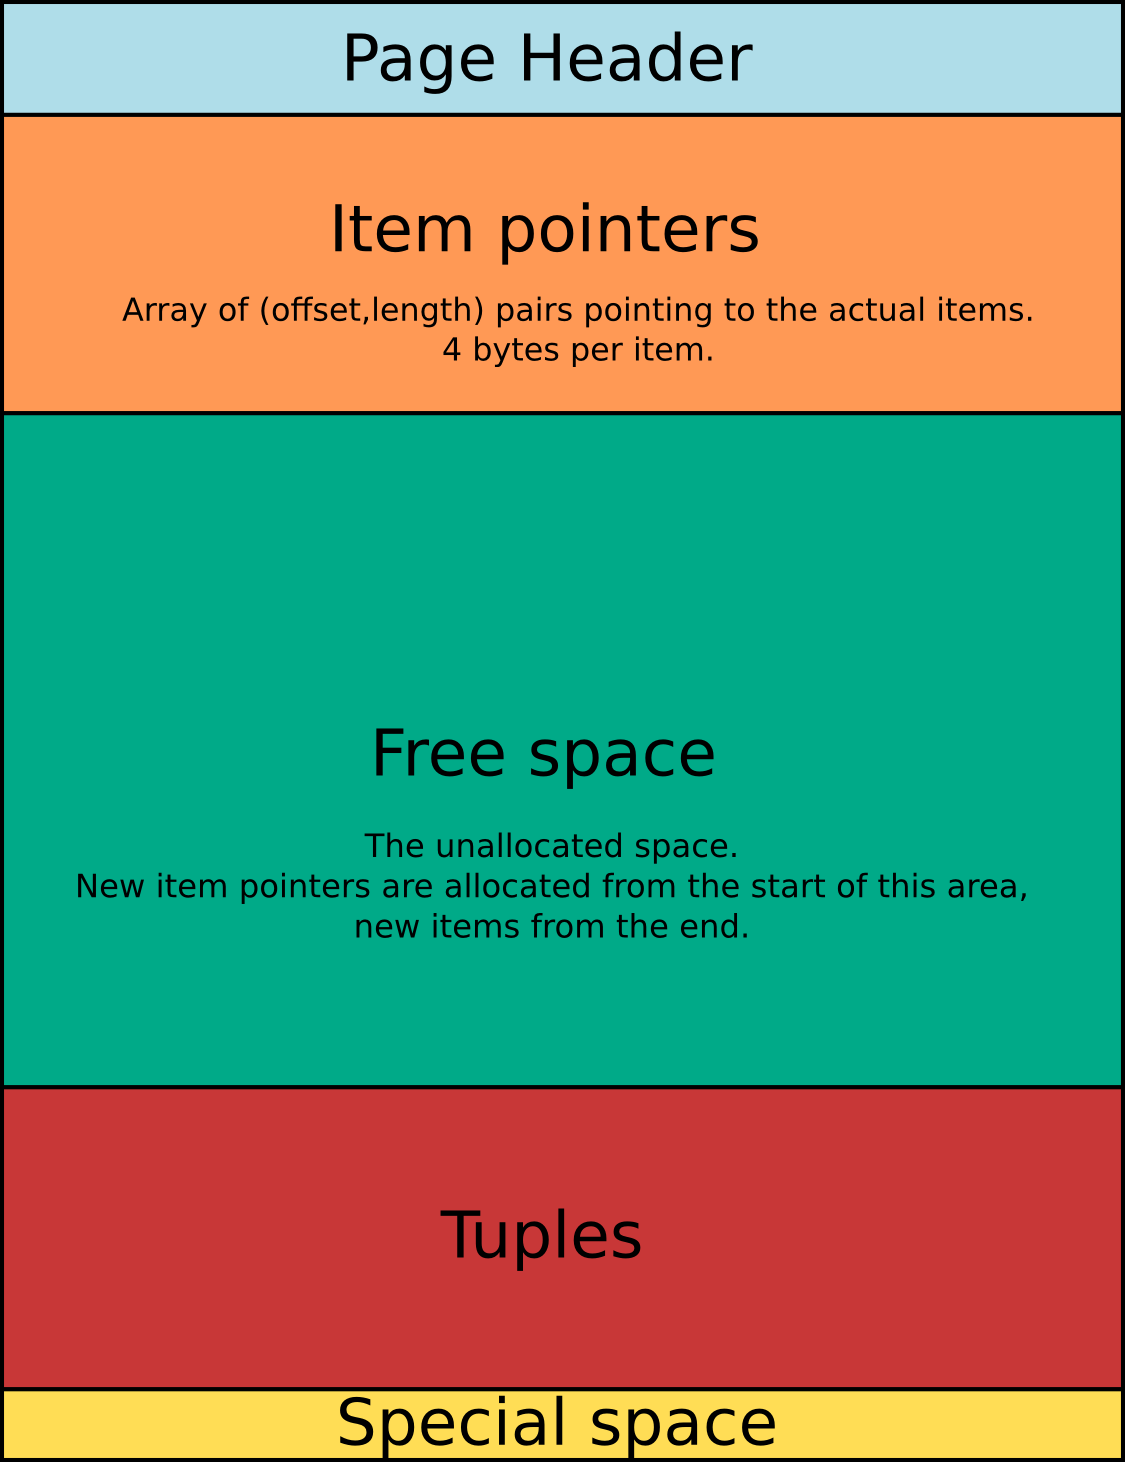
\includegraphics[scale=0.35]{images/index_page_01.png}

\caption{Index page}
\label{fig:INDEX01} 
\end{center}

\end{figure}

A data page starts with a header of \index{Data pages,header}24 bytes. After the 
header there are the item pointers, which size is usually 4 bytes. Each item 
pointer\index{Item pointers} is an array of pairs composed by the offset and the length 
of the item which ponints the physical tuples in the page's bottom.\newline 

The page header holds the information for the page's generic space management as shown 
in figure \ref{fig:HEADERPAG01}. 


\begin{figure}[H]
\begin{center}

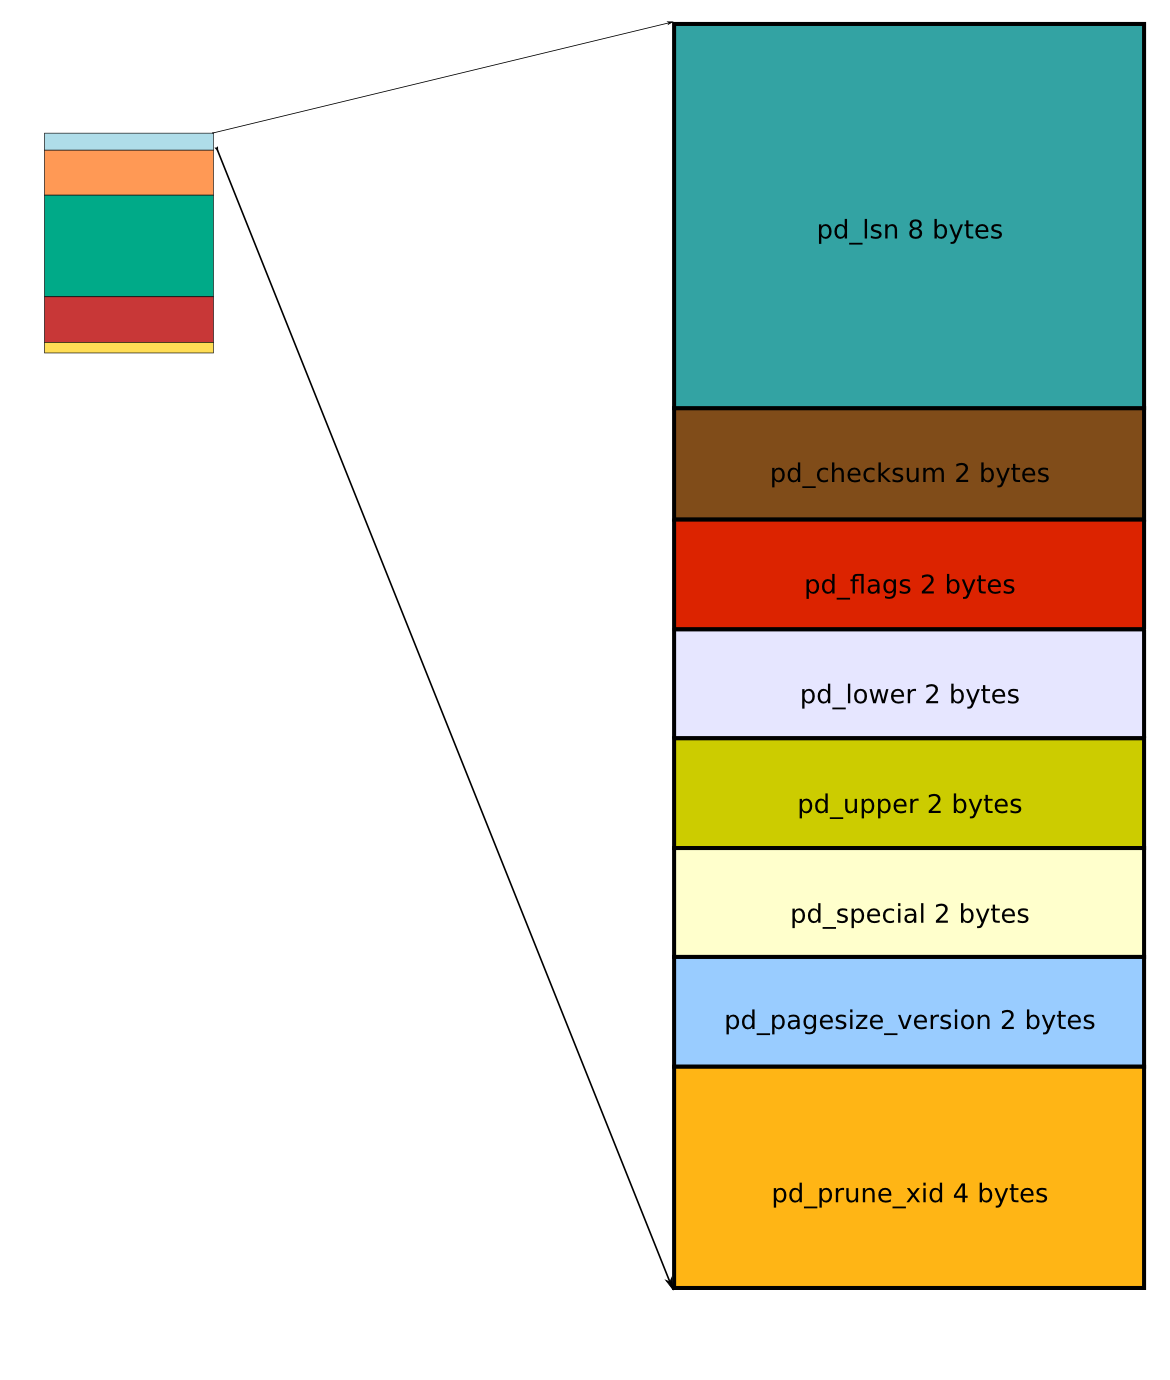
\includegraphics[scale=0.55]{images/header_page_01.png}

\caption{Page header}
\label{fig:HEADERPAG01} 
\end{center}

\end{figure}
\begin{itemize}
 \item \textbf{pd\_lsn} identifies the xlog record for last page's change.  The 
buffer manager uses the  LSN for enforcing the WAL mechanism. A dirty buffer is not 
dumped to the disk until the xlog has been flushed at least as far as the page's LSN.
\item \textbf{pd\_checksum} stores the page's checksum if is enabled.
\item \textbf{pd\_flags} is used to store the page's various flags 
\item \textbf{pg\_lower} is the offset to the start of the free space
\item \textbf{pg\_upper} is the offset to the end of the free space
\item \textbf{pg\_special} is the offset to the start of the special space
\item \textbf{pd\_pagesize\_version} is the page size and the page version packed 
together in a single field. 
\item \textbf{pg\_prune\_xid} is a hint field to determine if the tuple's pruning is 
useful. Is set only on the heap pages.

\end{itemize}

The pd\_checksum \index{Page checksum}field replaces the pd\_tli field present in the page 
header until PostgreSQL 9.2 which was used to track the xlog records across the timeline id. 
\newline 

The page's checksum is a new 9.3's feature which can detects the page corruption. It can be enabled only 
when the data area is initialised with initdb.\newline

The offset fields, pg\_lower, pd\_upper and the optional pd\_special, are 2 bytes long limiting the 
max page size to 32KB.\newline

The field for the page version\index{Page version} was introduced with PostgreSQL 7.3. 
Table \ref{tab:PGPAGEVERSION} shows the page version number for the major versions.

\begin{table}[h]
  \begin{tabular}{cc}
    PostgreSQL version & Page version\\
    \hline
    \textgreater \space 8.3  &  4\\
    8.1,8.2  &  3\\
    8.0  &  2\\
    7.4,7.3  &  1\\
    \textless \space 7.3  &  0\\
    
    
  \end{tabular}
  \caption{\label{tab:PGPAGEVERSION}PostgreSQL page version}
\end{table}

\section{Tuples}\index{Tuples}
\label{sec:TUPLES}
The tuples are the fundamental storage unit in PostgreSQL. They are organised as array of items which kind 
is initially unknown, the datum. Each tuple have a fixed header of 23 bytes as shown in the figure 
\ref{fig:TUPLES01}.\newline

\begin{figure}[H]
\begin{center}

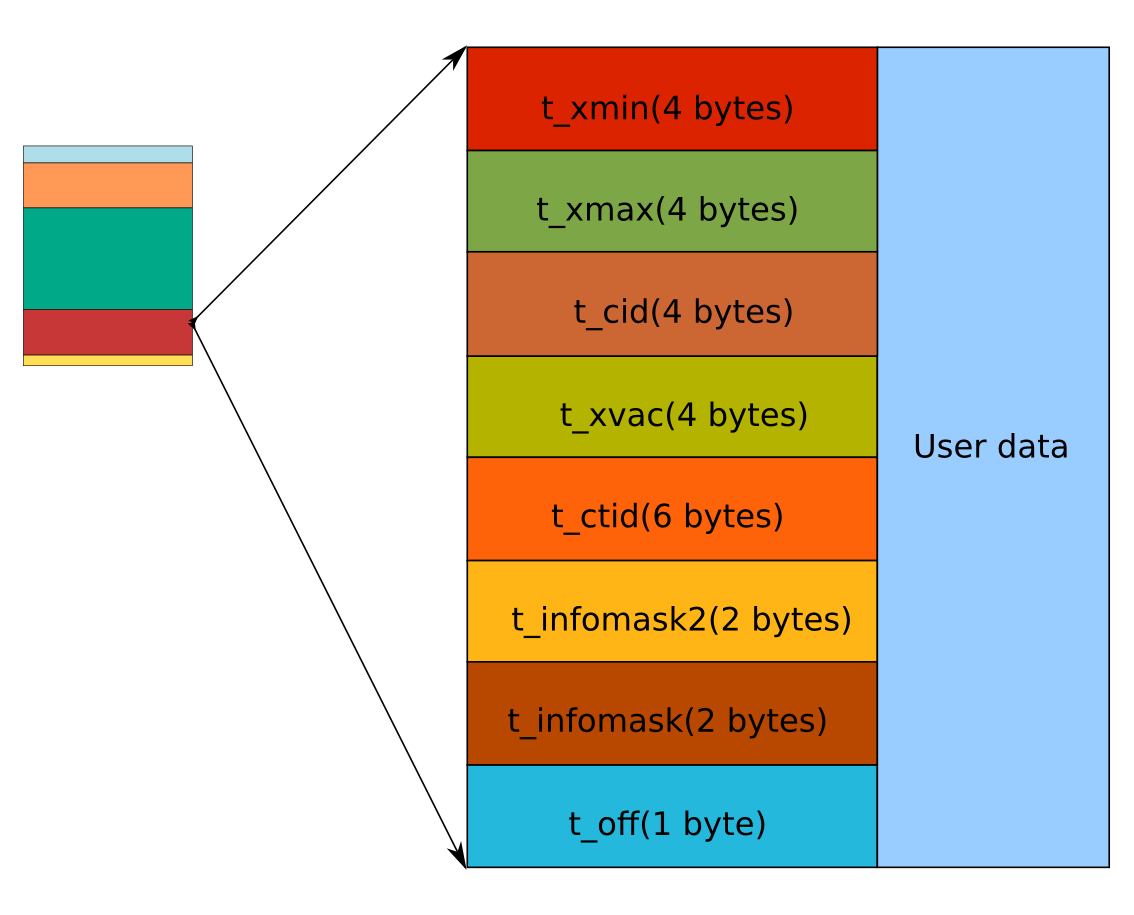
\includegraphics[scale=0.55]{images/tuples_01.png}

\caption{Tuple structure}
\label{fig:TUPLES01} 
\end{center}

\end{figure}

The fields t\_xmin\index{t\_xmin} and t\_xmax\index{t\_xmax} are used to track the tuple's visibility as 
seen in \ref{sec:MVCC}. The field t\_cid\index{t\_cid} is a ``virtual'' field and is used either for cmin 
and cmax. \newline

The field t\_xvac\index{t\_xvac} is used by VACUUM when moving the rows, according with the source code's 
comments in src/include/access/htup\_details.h this field is used only by the old style VACUUM FULL. 
\newline

The field t\_cid\index{t\_cid} is the tuple's physical location identifier. Is composed by a couple of 
integers representing the page number and the tuple's index along the page. When a new tuple is created 
t\_cid is set to the actual row's value. When the tuple is updated the this 
value changes to the new tuple's version location. This field is used in pair with t\_xmax to check if 
the tuple is the last version. The two infomask fields are used to store various flags like the presence of 
the tuple's OID or if the tuple have NULL values. The last field t\_off is used to set the offset to the 
actual tuple's data. This field's value is usually zero if the table doesn't have NULLable fields or is 
created WITHOUT OIDS. If the tuples have the OID and or a NULLable fields, the object identifier and 
a NULL bitmap are stored immediately after the tuple's header. The bitmap if present begins just after the 
tuple's header and consumes enough bytes to have one bit per data column. The OID if present is stored 
after the bitmap and consumes 4 bytes. The tuple's data is a stream of composite data described by the 
composite model stored in the system catalogue. 


\section{TOAST}\index{TOAST}
\label{sec:TOAST}
The oversize attribute storage technique is the PostgreSQL implementation for storing the data 
which overflows the page size. PostgreSQL does not allow the tuples spanning multiple pages. However is 
possible to store large amount of data which is compressed or split in multiple rows in an external 
TOAST table. The mechanism is completely transparent from the user's point of view.\newline

The storage model treats the fixed length, like the integers, and the variable length types, like text, in 
a different way. The fixed length types which cannot produce large data are not processed through the TOAST 
routines. The variable length types are TOASTable if the first 32-bit word of any stored value contains the 
total length of the value in bytes (including itself).

The kind of the TOAST is stored in the first two bits\footnote{On the big-endian architecture those are the 
high-order bits; on the little-endian those are the low-order bits} of the varlena\index{varlena} length 
word. When both bits are zero then the attribute is an unTOASTed data type. In the remaining bits is stored 
the datum size in bytes including the length word.\newline

If the first bit is set then the value have only a single-byte header instead of the four byte header. 
In the remaining bits is stored the total datum size in bytes including the length byte. This scenario 
have a special case uf the remaining bits are all zero. This means the value is a pointer to an out of line 
data stored in a separate TOAST table which structure is shown in figure \ref{fig:TOAST01}.\newline

Finally, whether is the first bit,  if the second bit is set then the corresponding datum is compressed and 
must be decompressed before the use.\newline

Because the TOAST usurps the first two bits of the varlena length word it limits the max stored size to 1 
GB  \begin{math} (2^{30} -1 bytes) \end{math} .

\begin{figure}[H]
\begin{center}

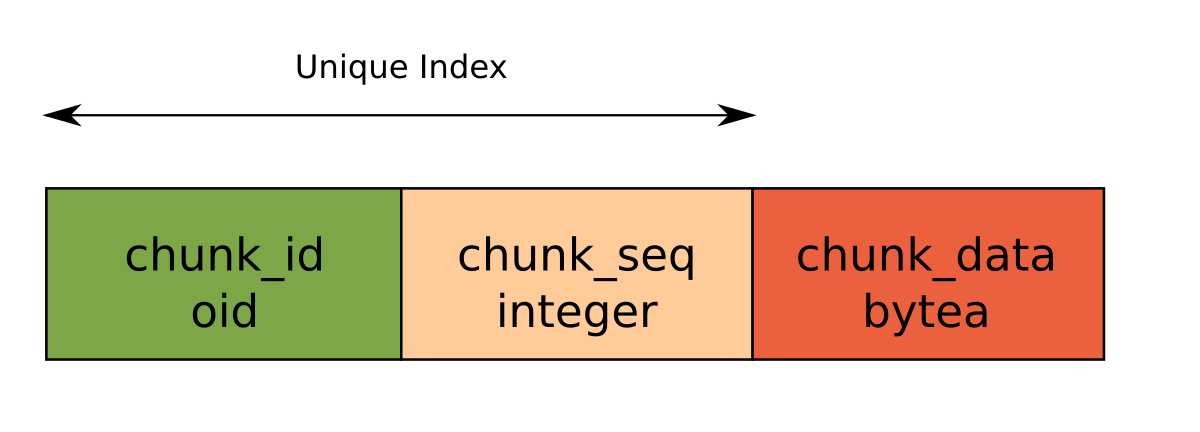
\includegraphics[scale=0.55]{images/toast_01.png}

\caption{Toast table structure}
\label{fig:TOAST01} 
\end{center}

\end{figure}

The toast table is composed by three fields. The chunk\_id is an OID used to store the chunk identifiers. 
The chunk\_seq is an integer which stores the chunk orders. The chunk\_data is a bytea field containing the 
the actual data converted in a binary string.\newline 

The chunk size is normally 2k and is controlled at compile time by the symbol\newline 
TOAST\_MAX\_CHUNK\_SIZE. The TOAST code is triggered by the value\newline  TOAST\_TUPLE\_THRESHOLD, also 2k 
by default. When the tuple's size is 
bigger than \newline TOAST\_TUPLE\_THRESHOLD then the TOAST routines are triggered.\newline

The TOAST\_TUPLE\_TARGET, default 2 kB, governs the compression's behaviour. PostgreSQL will compress the 
datum to achieve a final size lesser than \newline TOAST\_TUPLE\_TARGET. Otherwise the out of line storage 
is used.

TOAST offers four different storage strategies. Each strategy can be changed per column using the  ALTER 
TABLE SET STORAGE statement.
\begin{itemize}

\index{TOAST, storage strategies}
\item  PLAIN prevents either compression or out-of-line storage; It's the only storage available 
for fixed length data types.

\item  EXTENDED allows both compression and out-of-line storage. It is the default for most 
TOAST-able data types. Compression will be attempted first, then out-of-line storage if the row is 
still too big.

\item  EXTERNAL allows out-of-line storage but not compression. 

\item  MAIN allows compression but not out-of-line storage. Actually the out-of-line storage is 
still performed as last resort.

\end{itemize}

The out of line storage\index{TOAST, out of line storage} have the advantage of leaving out the 
stored data from the row versioning; if the TOAST data is not affected by the update there will be 
no dead row for the TOAST data. That's possible because the varlena is a mere pointer to the chunks 
and a new row version will affect only the pointer leaving the TOAST data unchanged.\newline
The TOAST table are stored like all the other relation's in the pg\_class table, the associated 
table can be found using a self join on the field reltoastrelid.\newline


\section{Tablespaces}\index{tablespaces,physical}
\label{sub:TBS-PHYSICAL}
PostgreSQL implements the tablespaces with the symbolic links. Inside the directory \$PGDATA/pg\_tblspc 
there are the links to the physical location. Each link is named after the tablespace's OID. Therefore the 
tablespaces are available only on the systems with the symbolic link support.\newline

Before the version 8.4 the tablespace symbolic link pointed directly to the referenced directory. This was 
a race condition when upgrading in place because the the location could clash with the upgraded cluster. 
From the version 9.0, the tablespace creates a sub directory directory in the tablespace location which 
is after the major version and the system catalogue version number. 
\newline

\begin{verbatim}

postgres@tardis:~$ ls -l /var/lib/postgresql/pg_tbs/ts_test
total 0
drwx------ 2 postgres postgres 6 Jun  9 13:01 PG_9.3_201306121

\end{verbatim}

The sub directory's name is a combination of the capital letters PG followed by the major version, 
truncated to the first two numbers, and the catalogue version number stored in the control file.\newline



\begin{verbatim}
postgres@tardis:~$ export PGDATA=/var/lib/postgresql/9.3/main
postgres@tardis:~$ /usr/lib/postgresql/9.3/bin/pg_controldata 
pg_control version number:            937
Catalog version number:               201306121
Database system identifier:           5992975355079285751
Database cluster state:               in production
pg_control last modified:             Mon 09 Jun 2014 13:05:14 UTC
.
.
.
WAL block size:                       8192
Bytes per WAL segment:                16777216
Maximum length of identifiers:        64
Maximum columns in an index:          32
Maximum size of a TOAST chunk:        1996
Date/time type storage:               64-bit integers
Float4 argument passing:              by value
Float8 argument passing:              by value
Data page checksum version:           0



PG_{MAJOR_VERSION\}_{CATALOGUE_VERSION_NUMBER}

\end{verbatim}



Inside the container directory the data files are organised in the same way as in base directory.
\ref{sec:PGDATA}.\newline

Moving a tablespace to another physical location it's not complicated but the cluster needs to be shut down.
With the cluster stopped the container directory can be safely copied to the new location. The receiving 
directory must have the same permissions  like the origin's. The symbolic link must be recreated to point 
to the new physical location. At the cluster's start the change will be automatically resolved from 
the symbolic link.\newline

Until PostgreSQL 9.1 the tablespace location was stored into the field spclocation in the system table 
pg\_tablespace\index{pg\_tablespace}. From the version 9.2 the spclocation field is removed and the 
tablespace's location is resolved on the fly using the function 
pg\_tablespace\_location(tablespace\_oid).\newline

This function can be used to query the system catalogue about the tablespaces. In this simple example the 
query returns the tablespace's location resolved from the OID. 

\begin{lstlisting}[style=pgsql]
postgres=# 
                SELECT 
                        pg_tablespace_location(oid),
                        spcname 
                FROM 
                        pg_tablespace
                ;
        
       pg_tablespace_location       |  spcname   
------------------------------------+------------
                                    | pg_default
                                    | pg_global
 /var/lib/postgresql/pg_tbs/ts_test | ts_test
(3 rows)

\end{lstlisting}

Because the function pg\_tablespace\_location returns the empty string for the system tablespaces, a better 
approach is combining the CASE construct with the function current\_settings and build the absolute path 
for the system tablespaces.

\begin{lstlisting}[style=pgsql]
 postgres=# SELECT current_setting('data_directory');
       current_setting        
------------------------------
 /var/lib/postgresql/9.3/main
(1 row)

postgres=# 
SELECT 
        CASE
                WHEN 
                                pg_tablespace_location(oid)=''
                        AND     spcname='pg_default'
                THEN
                        current_setting('data_directory')||'/base/'
                WHEN 
                                pg_tablespace_location(oid)=''
                        AND     spcname='pg_global'
                THEN
                        current_setting('data_directory')||'/global/'
        ELSE
                pg_tablespace_location(oid)
        END
        AS      spclocation,
                
        spcname 
FROM 
        pg_tablespace;
             spclocation              |  spcname   
--------------------------------------+------------
 /var/lib/postgresql/9.3/main/base/   | pg_default
 /var/lib/postgresql/9.3/main/global/ | pg_global
 /var/lib/postgresql/pg_tbs/ts_test   | ts_test
(3 rows)

\end{lstlisting}

Another useful function the pg\_tablespace\_databases(tablespace\_oid) can help us to find the databases 
with the relations on a certain tablespace.\newline

The following example uses this function again with a CASE construct for building the database having 
objects on a specific tablespace, in our example the ts\_test created in \ref{sub:TBS-LOGICAL}.\newpage
\begin{lstlisting}[style=pgsql]
 db_test=# 
 SELECT
        datname,
        spcname,
        CASE
                WHEN 
                                pg_tablespace_location(tbsoid)=''
                        AND     spcname='pg_default'
                THEN
                        current_setting('data_directory')||'/base/'
                WHEN 
                                pg_tablespace_location(tbsoid)=''
                        AND     spcname='pg_global'
                THEN
                        current_setting('data_directory')||'/global/'
        ELSE
                pg_tablespace_location(tbsoid)
        END
        AS      spclocation
FROM
        pg_database dat,
        (
                SELECT
                        oid as tbsoid,
                        pg_tablespace_databases(oid) as datoid,
                        spcname 
                FROM 
                        pg_tablespace where spcname='ts_test'
        ) tbs
WHERE
        dat.oid=tbs.datoid
;
 datname | spcname |            spclocation             
---------+---------+------------------------------------
 db_test | ts_test | /var/lib/postgresql/pg_tbs/ts_test
(1 row)

\end{lstlisting}



\section{MVCC} \label{sec:MVCC}\index{MVCC} 
The multiversion concurrency control is used in PostgreSQL to implement the  transactional model seen in 
\ref{sec:TRANSACTION}.\newline

At logical level this is completely transparent to the user and the new row versions become visible 
after the commit, accordingly with the transaction isolation level. \newline

At physical level we have for each new row version, the insert's XID stored into the t\_xmin field which is 
used by the internal semantic to determine the row visibility. 

Because the XID is a 32 bit quantity, it wraps at 4 billions. When this happens theoretically all 
the tuples should suddenly disappear because they switch from in the current XID's past to its future in 
the well known XID wraparound failure,\index{XID wraparound failure}. In the old PostgreSQL versions this 
was a serious problem which forced the administrators to dump/reload the entire cluster into a freshly 
initialised new data area every 4 billion of transactions.\newline 

In PostgreSQL 7.2 was introduced a new comparison method for the XID, the 
\begin{math}modulo-2^{32}\end{math} arithmetic. It was also introduced a special XID, the 
FrozenXID\footnote{The FrozenXID's value is 2. The docs of PostgreSQL 
7.2 also mention the BootstrapXID which value is 1} assumed as always in the past. With the new 
comparison method, for any arbitrary XID exists 2 billion of transactions in the future and 2 billion 
transactions in the past.\newline

When the age of the tuple's t\_xmin becomes old the periodic VACUUM\index{VACUUM} freezes the ageing tuple 
changing its t\_xmin to the FrozenXID always in the past. In the pg\_class and the pg\_database tables 
there are  two dedicated fields to track the age of the oldest XID. The value stored in those tables 
have little meaning if not processed through the function age() which shows the number of transactions 
between the current XID and the value stored in the system catalogue. \newline

This following query returns all the databases, the corresponding datfrozenxid and the XID's age.\newpage

\begin{lstlisting}[style=pgsql]
 postgres=# 
        SELECT 
                datname,
                age(datfrozenxid),
                datfrozenxid 
        FROM 
                pg_database;
    datname    | age  | datfrozenxid 
---------------+------+--------------
 template1     | 4211 |          679
 template0     | 4211 |          679
 postgres      | 4211 |          679
 db_test       | 4211 |          679

\end{lstlisting}

When a tuple's age is more than 2 billions the tuple simply disappears  from the cluster. Before the 
version 8.0 there was no alert or protection against the XID wraparound failure. Since then it was 
introduced a passive mechanism which emits messages in the activity log when the age of datfrozenxid 
is less than ten million transactions from the wraparound point.

A message like this is quite serious and should not be ignored.
\begin{smallverbatim}
WARNING:  database "test_db" must be vacuumed within 152405486 transactions
HINT:  To avoid a database shutdown, execute a database-wide VACUUM in 
"test_db".
\end{smallverbatim}

The autovacuum daemon in this case acts like a watchdog and starts vacuuming the tables with ageing 
tuples even  if autovacuum is turned off in the cluster. There is another protection, quite radical, 
if for some reasons one of the database's datfrozenxid is at one million transactions from the 
wraparound point. In this case the cluster shuts down and refuse to start again. The only option in 
this case is to run the postgres process in single-user backend and execute the VACUUM on the 
affected relations.\newline

The debian package's configuration is quite odd, putting the configuration files in the /etc/postgresql 
instead of the data area. The following example is the standalone backend's call for the debian's packaged 
default cluster main.

\begin{verbatim}

postgres@tardis:~/tempdata$ /usr/lib/postgresql/9.3/bin/postgres \
--single -D /var/lib/postgresql/9.3/main/base/ \
--config-file=/etc/postgresql/9.3/main/postgresql.conf

PostgreSQL stand-alone backend 9.3.5
backend> 

\end{verbatim}

The database interface in single user mode and does not have all the sophisticated features 
like the client psql. Anyway with a little knowledge of SQL it's possible to find the database(s) 
causing the shutdown and fix it.
\index{postgres, single user mode}\index{XID wraparound failure, fix}

\begin{verbatim}
backend> SELECT datname,age(datfrozenxid) FROM pg_database ORDER BY 2 DESC;

1: datname     (typeid = 19, len = 64, typmod = -1, byval = f)
2: age (typeid = 23, len = 4, typmod = -1, byval = t)
----
1: datname = "template1" (typeid = 19, len = 64, typmod = -1, byval = f)
2: age = "2146435072"  (typeid = 23, len = 4, typmod = -1, byval = t)
----
1: datname = "template0" (typeid = 19, len = 64, typmod = -1, byval = f)
2: age = "10"  (typeid = 23, len = 4, typmod = -1, byval = t)
----
1: datname = "postgres"  (typeid = 19, len = 64, typmod = -1, byval = f)
2: age = "10"  (typeid = 23, len = 4, typmod = -1, byval = t)
----

\end{verbatim}

The age function shows how old is the last XID not yet frozen. In our example the template1
database have an age of 2146435072, one million transactions to the wraparound. We can then exit 
the backend with CTRL+D and restart it again in the in single user mode specifying the database 
name. A VACUUM will get rid of the problematic xid.

\begin{verbatim}
postgres@tardis:~/tempdata$ /usr/lib/postgresql/9.3/bin/postgres \
--single -D /var/lib/postgresql/9.3/main/base/ \
--config-file=/etc/postgresql/9.3/main/postgresql.conf \
template1
                                
backend> SELECT current_database();
1: current_database (typeid = 19, len = 64, typmod = -1, byval = f)
----
1: current_database = "template1" (typeid = 19, len = 64, typmod = -1, byval = f)
----

backend> VACUUM FREEZE;
\end{verbatim}

This procedure must be repeated for any database with very old XID.\newline

Because the new rows generation at update time, this can lead to an unnecessary table and index bloat.
PostgreSQL with the Heap Only Tuples (HOT)\index{HOT strategy} strategy can limit the unavoidable bloat 
caused by the updates. HOT's main goal is to keep the new row versions into the same page. 

The MVCC is something to consider at design time. Ignoring the way PostgreSQL manages the physical tuples 
can result in data bloat and lead in general to poor performances.
